% Para iniciar una sección debe escribirse
%\section{Nombre de la sección}
% Lo anterior inmediatamente creará la sección y la numerará.

\section*{Objetivos}
\subsection*{Generales}
\begin{itemize}
    \item Diseñar y construir una calculadora capaz de realizar operaciones aritméticas básicas capaz de desplegar la información en formato base 10
\end{itemize}

\subsection*{Específicos}
\begin{itemize}
    \item Diseñar múltiples circuitos combinacionales para obtener un resultado único en conjunto
    \item Implementar un circuito de lógica combinacional capaz de realizar operaciones aritméticas simples utilizando únicamente compuertas lógicas
    \item Optimizar el uso de compuertas mediante técnicas distintas al uso de Mapas de Karnaugh
    \item Contrastar los diseños teóricos con los resultados experimentales de los circuitos implementados físicamente
\end{itemize}

\section{Introducción}

\subsection{Aritmética binaria}
Los dispositivos digitales se basan en operaciones con numeración \emph{base 2} para obtener los resultados, incluso si la interfaz de usuario tuviese otro 
formato (numérico decimal, en base a gráficos o imágenes, etc.). Las operaciones aritméticas en \emph{base 2} cumplen con los mismos teoremas y reglas que se
utilizan en base 10, pero poseen la ventaja de tener más simplificaciones debido a la limitada cantidad de dígitos disponibles. Consulte su libro de
texto\footnote{Mano, Morris. Digital Design, 5th edition} para recapitular lo anteriormente descrito.

% \begin{figure}[H]
%     \centering
%     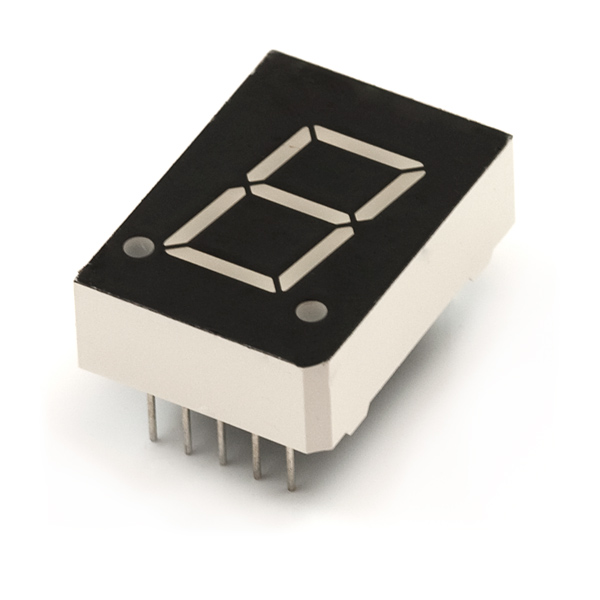
\includegraphics[scale=0.3]{images/7SegmentDisplay.jpg}
%     \caption{Display de 7 segmentos}
%     \label{Fig:SevenSegment}
% \end{figure}


\pagebreak

\section{Desarrollo Experimental}
\subsection{Materiales y Equipo}

Cada grupo debe llevar su material y equipo de trabajo durante las prácticas. Pregunte a su profesor qué \emph{Equipo de Laboratorio} puede ser prestado
de parte del laboratorio de instrumentación. El laboratorio de instrumentación no tiene disponibilidad de ningún elemento de la lista \emph{Materiales}.

\subsubsection*{Materiales}
\begin{itemize}
    \item 1x dip-switch de 7 posiciones (o más)
    \item 7x pulsadores (si no consiguiesen el dip-switch de 4 posiciones)
    \item 1x fuente de alimentación (ver apartado anterior con todas las alternativas)
    \item 2x capacitores electrolíticos de 47 $\mu$F 16V
    \item 2x capacitores cerámicos de 100nF 25V
    \item 6x resistencias de 1 k$\ohm$
    \item 2x LEDs de cualquier color
    \item 1x Display de 7 segmentos de \textbf{ánodo común} de cualquier color
    \item 7x Resistencias $220 \ohm \leq R \leq 1 k\ohm$
    \item 6x metros de alambre para protoboard calibre 22. Compren al menos 2 colores para los 6 metros. \textbf{No usen \emph{UTP}}, aunque eso les quieran vender.
    \item 1x Circuito Integrado 74LS47 (decodificador BCD a Display 7 segmentos ánodo común)
    \item Las compuertas lógicas a utilizar dependen del diseño final de cada grupo (AND, OR, NOT, XOR, NAND, XNOR)
\end{itemize}


\subsubsection*{Equipo de Laboratorio}
\begin{itemize}
    \item 1x Pinzas delgadas
    \item 1x Cortaalambres
    \item 1x Pelador de alambres para calibre 22 (opcional)
    \item 1x Tijeras pequeñas o cortauñas (si no tienen pela alambres)
    \item 1x Protoboard de al menos 2 galletas (puede juntar 2 protoboards de 1 galleta)
    \item 1x Multímetro digital para medir voltaje
\end{itemize}

\subsection{Procedimiento}
\subsubsection{Fuente de alimentación}
Utilice la misma fuente de alimentación que en la Práctica \#1.

\subsubsection{Calculadora básica}
Se debe diseñar una calculadora con entradas a través de una interfaz binaria (dip-switch o pulsadores) que despliegue el resultado de la
operación en un display de 7 segmentos. Las operaciones a realizar son:
\begin{itemize}
    \item Suma 
    \item Resta sin signo
    \item Indicar Overflow/Underflow con un LED
\end{itemize}

\vspace{14pt}


\subsection{Interfaz de usuario}
El método de entrada son 2 variables de 3 bits ($A_0, A_1, A_2, B_0, B_1, B_2$) a través de \emph{dip-switch} o pulsadores. Además, debe existir
un interruptor dedicado para seleccionar si la operación a realizar es \emph{suma} o \emph{resta sin signo}.
Debido a que el CI 74LS47 despliega caracteres no alfanuméricos con para valores entre 0x0A y 0x0F, esto se tomará en consideración y 
no será necesario hacer ninguna corrección para mostrar el valor adecuado en el rango de 0x0A - 0x0F.

\section{Resultados esperados}
\subsection{Funcionamiento completo}
Utilice la simplificación de \emph{full adders} para la realización de la práctica (implementados con compuertas), no realice las reducciones a través de Mapas de Karnaugh (o si lo desea, puede
morir en el intento).

\pagebreak

\section{Bonus}
Como tendrán tiempo extra para realizar el diseño de la práctica (debido a la semana de Congreso Estudiantil), esta sección se coloca como un \emph{reto extra} 
que \textbf{no es obligatorio} hacer. Sin embargo, esta sección puede exonerarlos de una parte (o de todo) el segundo parcial si el funcionamiento es correcto
y cumple con todos los requisitos solicitados. Todo debe entregarse en el reporte y funcionando físicamente en protoboard el \textbf{lunes 07/10/2019}.

\subsection{Multiplicador decimal} \label{sec:Multiplicador}
\emph{Equivalente al 40\% del Segundo Examen Parcial}
\vspace{14pt}

Utilizando \textbf{dos display de 7 segmentos} desplegar el producto de dos variables de 3 bits (cada una). Puede utilizar
únicamente compuertas lógicas (AND, OR, NOT, XOR, NAND, XNOR) y 2 driver de display de 7 segmentos (74LS47). El resultado debe mostrarse en \emph{base 10}
sin utilizar los caracteres hexacecimales (0x0A, 0x0B, 0x0C, 0x0D, 0x0F).

\subsection{Divisor decimal entero}
\emph{Equivalente al 60\% del Segundo Examen Parcial}
\vspace{14pt}

Para que esta sección tenga validez, el multiplicador (sección \ref{sec:Multiplicador}) debió haber sido implementado a cabalidad. El divisor decimal debe incluir 
una entrada de 4 bits para el dividendo y 2 bits para el divisor. El diseño debe incluir únicamente compuertas lógicas (AND, OR, NOT, XOR, NAND, XNOR) y
2 driver de display de 7 segmentos (74LS47). El resultado debe mostrarse en \emph{base 10} sin utilizar los caracteres hexadecimales (0x0A, 0x0B, 0x0C, 0x0D, 0x0F).